\begin{figure}[H]
    \begin{subfigure}[t]{0.5\textwidth}
        \caption{}
        \centering
        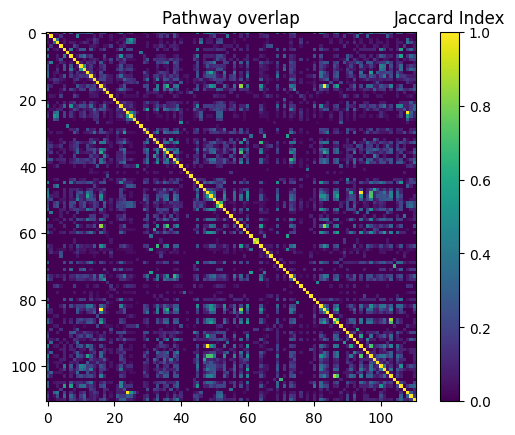
\includegraphics[width=0.8\textwidth]{./extended_plots/jaccard_mat_sub.png}        
    \end{subfigure}
    \begin{subfigure}[t]{0.5\textwidth}
        \caption{}
        \centering
        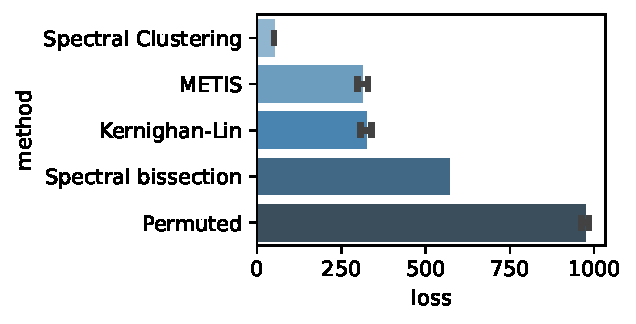
\includegraphics[width=0.8\textwidth]{./extended_plots/partitioning_losses.pdf}        
    \end{subfigure}
    \begin{subfigure}[t]{1\textwidth}
        \caption{}
        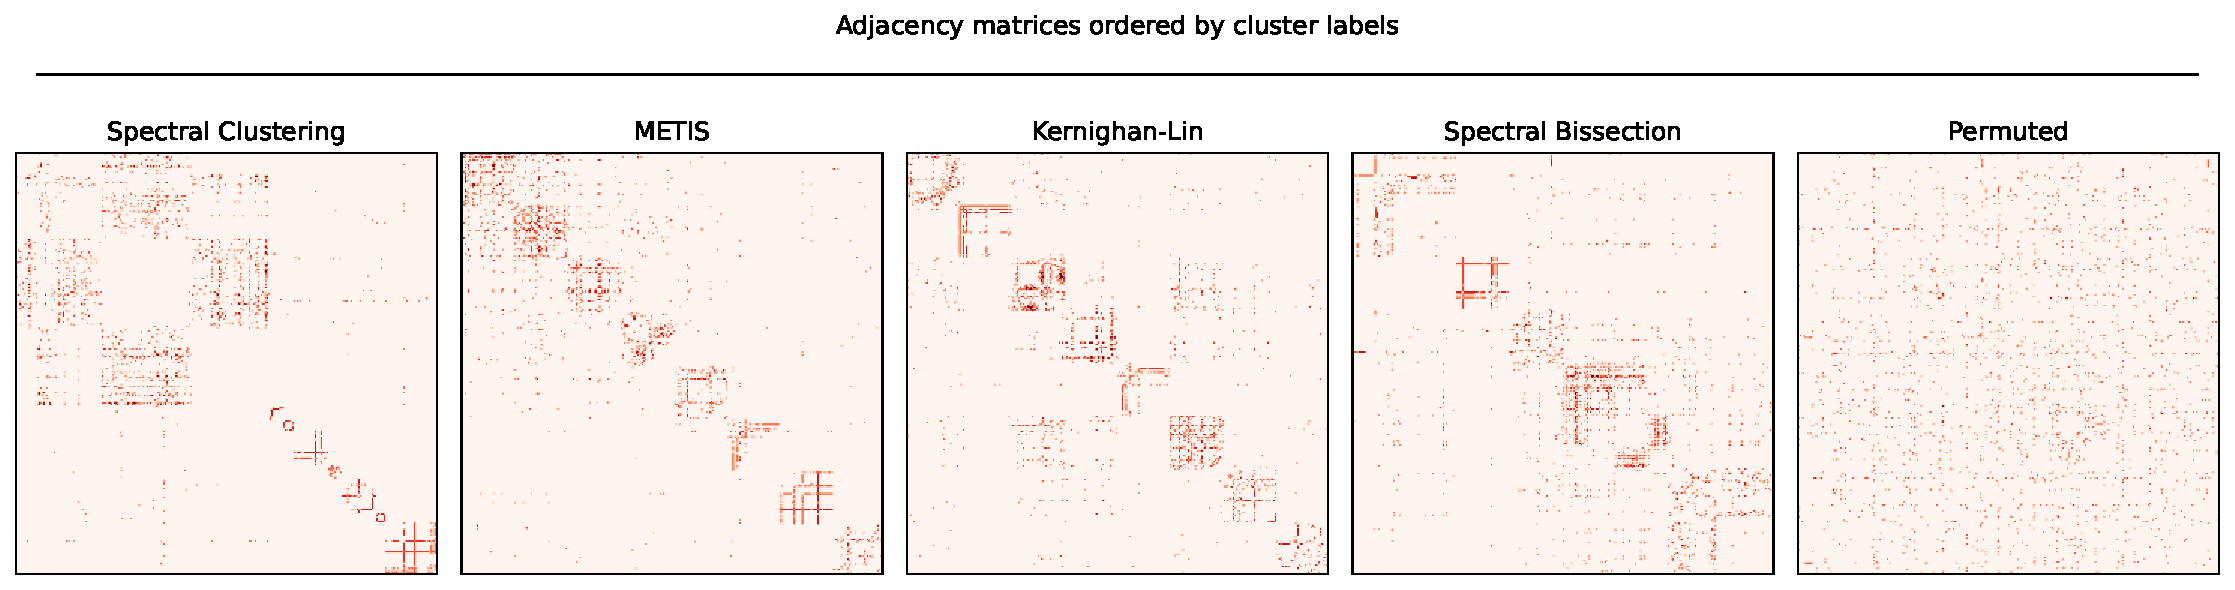
\includegraphics[width=\textwidth]{./extended_plots/adjacency_matrices_ordered_by_cluster_labels.pdf}        
    \end{subfigure}
    \begin{subfigure}[t]{0.33\textwidth}
        \caption{}
        \centering
        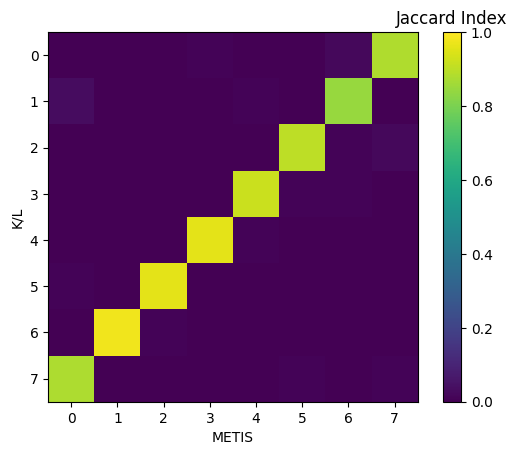
\includegraphics[width=0.8\textwidth]{./extended_plots/argmins_jaccard.png}        
    \end{subfigure}
    \begin{subfigure}[t]{0.33\textwidth}
        \caption{}
        \centering
        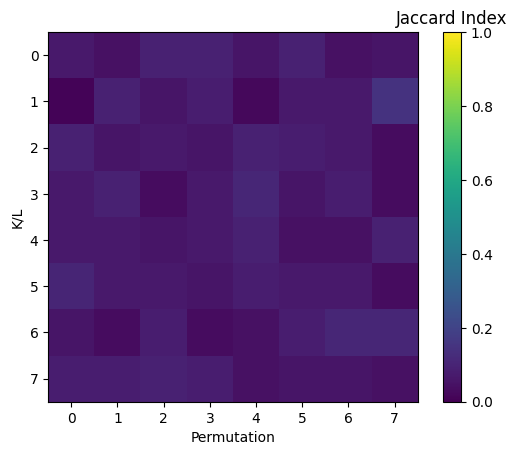
\includegraphics[width=0.8\textwidth]{./extended_plots/random_jaccard.png}        
    \end{subfigure}
    \begin{subfigure}[t]{0.33\textwidth}
        \caption{}
        \centering
        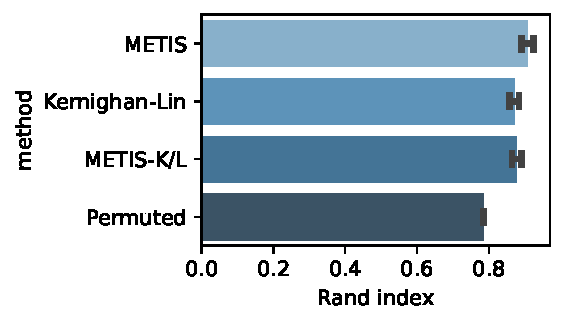
\includegraphics[width=0.8\textwidth]{./extended_plots/rand_indices.pdf}        
    \end{subfigure}
    \caption{
        \textbf{Benchmarking Partitioning and Clustering Algorithms for Gene-Pathway Grouping.}\\
    }
    \label{fig:benchmarking_clustering}
\end{figure}
\begin{itemize}
    \item[\textbf{(A)}] Jaccard indices quantifying overlap of genes for all 111 pathways in Figure~\ref{fig:main_excitatory}B (see Methods; Supplementary Text). 
    \item[\textbf{(B)}] Average loss (total cut size; see Methods) associated with applying each algorithm (spectral clustering (SC), METIS, Kernighan-Lin (K/L), spectral bisection (SB), or random permutation) to G (with 379 vertices; see Methods) over 1000 initiations (SC, random permutation) or $5 \times 10^5$ initiations (METIS, K/L). The SB implementation is deterministic and was run only once. Error bars indicate the standard deviation. 
    \item[\textbf{(C)}] Unweighted adjacency matrix for G sorted by labels assigned by the indicated algorithm. Red indicates the presence of an edge between two vertices. For each algorithm, labels corresponding to the best initiation (lowest loss) over 1000 initiations (SC, random permutation) or $5 \times 10^5$ initiations (METIS, K/L) are shown. 
    \item[\textbf{(D)}] Pairwise labeling consistency for the best K/L initiation and the best METIS initiation. Cluster labels corresponding to each are shown on the X- and Y-axes, respectively. Each color entry indicates the fraction of shared vertices per cluster across two initiations. Consistency is quantified using the Jaccard Index (JI). $\text{JI} = \frac{|A \cap B|}{|A \cup B|}$, where A and B are two sets (i.e., cluster A from initiation \#1 and cluster B from initiation \#2). 
    \item[\textbf{(E)}] Same as (D), but comparing the best K/L initiation against the best random permutation initiation. 
    \item[\textbf{(F)}] Average Rand index (RI) for all pairwise initiations from (B). “METIS,” “Kernighan-Lin,” and “Permuted” labels on the Y-axis indicate the average RI (consistency across two sets of labels) for all combinations of initiations within the specified algorithm. “METIS-K/L” indicates the average RI for all combinations of initiations across the METIS and Kernighan-Lin algorithms. Error bars indicate standard deviations. ($\text{RI} = \frac{\text{number of agreeing vertex pairs}}{\text{number of vertex pairs}}$).
\end{itemize}